\documentclass[tikz,margin=5mm]{standalone}
\usepackage{amssymb}
\usetikzlibrary{shapes.multipart,positioning,arrows,calc}
\tikzset{
    listnode/.style={
        rectangle split,rectangle split parts=2,draw,rectangle split horizontal,fill=yellow!15
    },
    startnode/.style={
        draw,minimum width=1cm,minimum height=.75cm
    }
}
\begin{document}
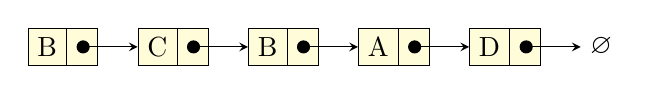
\begin{tikzpicture}[scale=5.0, >=stealth]
\node[listnode] (n1) {B};
\node[listnode,right=.5cm of n1] (n2) {C};
\node[listnode,right=.5cm of n2] (n3) {B};
\node[listnode,right=.5cm of n3] (n4) {A};
\node[listnode,right=.5cm of n4] (n5) {D};
\node[right=.5cm of n5] (n5x) {$\varnothing$};
\draw[*->] let \p1 = (n1.two), \p2 = (n1.center) in (\x1,\y2) -- (n2);
\draw[*->] let \p1 = (n2.two), \p2 = (n2.center) in (\x1,\y2) -- (n3);
\draw[*->] let \p1 = (n3.two), \p2 = (n3.center) in (\x1,\y2) -- (n4);
\draw[*->] let \p1 = (n4.two), \p2 = (n4.center) in (\x1,\y2) -- (n5);
\draw[*->] let \p1 = (n5.two), \p2 = (n5.center) in (\x1,\y2) -- (n5x);
\end{tikzpicture}



\end{document}
    


